\documentclass{article}

\usepackage{graphicx}
\graphicspath{ {./img/} }

\renewcommand{\thesubsection}{\alph{subsection})}

\title{IN2110 - Obligatorisk Oppgave 2a}
\author{Stian Carlsen Swärd (stiancsw)}

\begin{document}
\maketitle

\section{Oppgave 1}
\subsection{}
\begin{figure}[h]
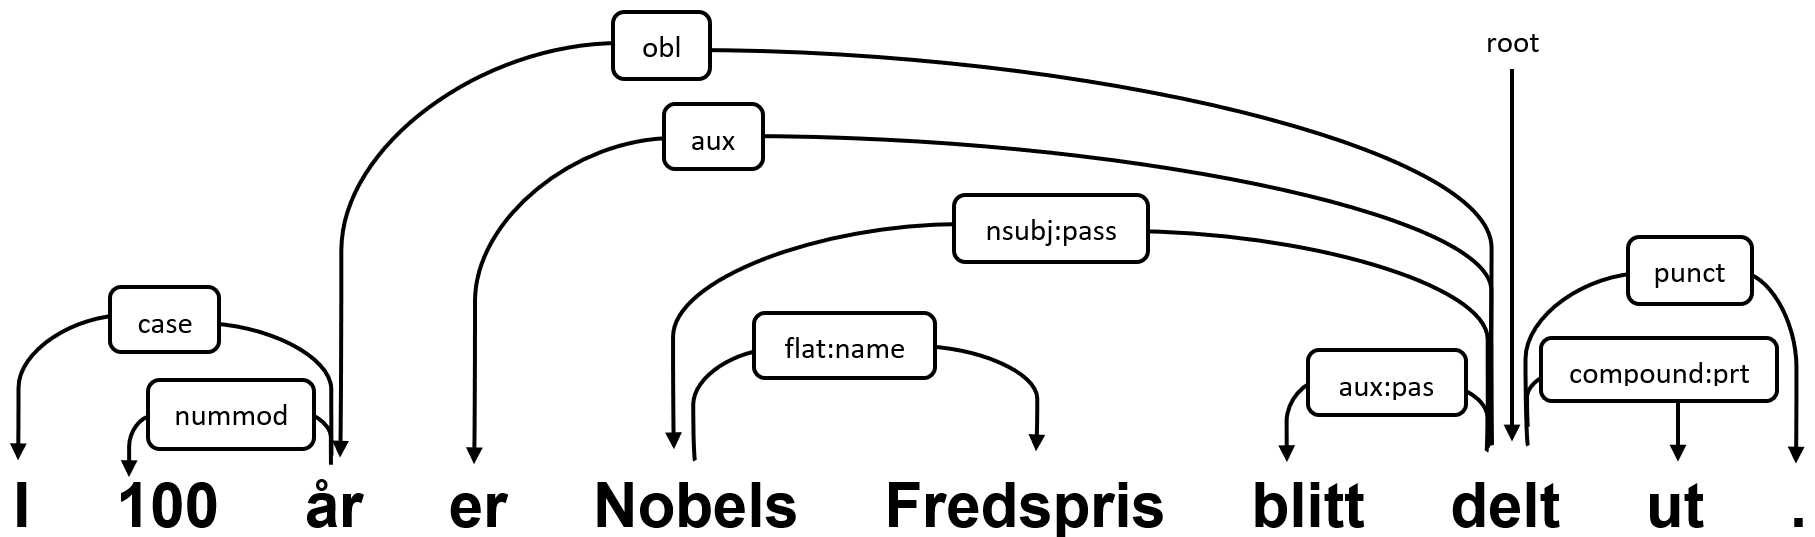
\includegraphics[scale=0.28]{1a-graph}
\caption{Dependensgraf for setningen i oppgavesettets Figur 1}
\end{figure}
\newpage
\subsection{}
Transisjonssekvens for setningen i oppgave 1a) ved bruk av arc-eager algoritmen\par

\begin{centering}
\begin{tabular}{ |c|c|c|c| }
\hline
OP &STACK & BUFFER & ARC \\
\hline
START & [ROOT]$_S$ & [I, ...]$_B$ & $Ø$ \\
\hline
SHIFT & [ROOT, I]$_S$ & [100, ...]$_B$ & $Ø$ \\
\hline
SHIFT & [ROOT, I, 100]$_S$ & [år, ...]$_B$ & $Ø$ \\
\hline
LA$_{nummod}$ & [ROOT, I]$_S$ & [år, ...]$_B$ & $A_1$ = \{(år, 100, $nummod$)\} \\
\hline
LA$_{case}$ & [ROOT]$_S$ & [år, ...]$_B$ & $A_2 = A_1 \cup$\{(år, I, $case$)\} \\
\hline
SHIFT & [ROOT, år]$_S$ & [er, ...]$_B$ & $A_2$ \\
\hline
SHIFT & [ROOT, år, er]$_S$ & [Nobels, ...]$_B$ & $A_2$ \\
\hline
SHIFT & [ROOT, ..., Nobels]$_S$ & [Fredspris, ...]$_B$ & $A_2$ \\
\hline
RA$_{flat:name}$ & [ROOT, ..., Fredspris]$_S$ & [blitt, ...]$_B$ & $A_3 = A_2\cup$\{(Nobels, Fredspris, $flat:name$)\} \\
\hline
REDUCE & [ROOT, ..., Nobels]$_S$ & [blitt, ...]$_B$ & $A_3$ \\
\hline
SHIFT & [ROOT, ..., blitt]$_S$ & [delt, ...]$_B$ & $A_3$ \\
\hline
LA$_{aux:pass}$ & [ROOT, ..., Nobels]$_S$ & [delt, ...]$_B$ & $A_4 = A_3\cup$\{(delt, blitt, $aux:pass$)\} \\
\hline
LA$_{nsubj:pass}$ & [ROOT, år, er]$_S$ & [delt, ...]$_B$ & $A_5 = A_4\cup$\{(delt, Nobels, $nsubj:pass$)\} \\
\hline
LA$_{aux}$ & [ROOT, år]$_S$ & [delt, ...]$_B$ & $A_6 = A_5\cup$\{(delt, er, $aux$)\} \\
\hline
LA$_{obl}$ & [ROOT]$_S$ & [delt, ...]$_B$ & $A_7 = A_6\cup$\{(delt, år, $obl$)\} \\
\hline
SHIFT & [ROOT, delt]$_S$ & [ut, .]$_B$ & $A_7$ \\
\hline
SHIFT & [ROOT, delt, ut]$_S$ & [.]$_B$ & $A_7$ \\
\hline
RA$_{compound:prt}$ & [ROOT, delt]$_S$ & [.]$_B$ & $A_8 = A_7\cup$\{(delt, ut, $compound:prt$)\} \\
\hline
SHIFT & [ROOT, delt, .]$_S$ & $Ø$ & $A_8$ \\
\hline
RA$_{punct}$ & [ROOT, delt]$_S$ & $Ø$ & $A_9 = A_8\cup$\{(delt, ., $punct$)\} \\
\hline
REDUCE & [ROOT]$_S$ & $Ø$ & $A_9$ \\
\hline
\end{tabular}
\end{centering}


Hovedforskjellene mellom arc og arc-eager er kompleksiteten ($O(n^5)$ vs $O(n^3)$), at arc-eager har en ekstra operasjon (REDUCE), samt at i arc kan ikke RIGHT-ARC-operasjonen utføres før vi har funnet alle tokens som er dependenser i en relasjon med dependensen i relasjonen vi jobber på.

\section{Oppgave 3}
\subsection{}
\textit{Se} \verb|oblig2a.py| \textit{for implementasjon av} \verb|attachment_score()|

\subsection{}
Tabell over UAS og LAS score for de ulike datasettene\newline

\begin{tabular}{ |c|c|c| }
\hline
Datasett & UAS & LAS \\
\hline
Bokmål & 0.893 & 0.798 \\
\hline
Nynorsk & 0.682 & 0.563 \\
\hline
NynorskLIA & 0.485 & 0.324 \\
\hline
\end{tabular}
\newpage
Vi ser, ikke overraskende,  at parseren scorer mye høyere på bokmålssettet enn på nynorsksettet, og høyere på nynorsksettet enn på det nynorske talespråksettet.\par


Vi printer ut \verb|nnlia_dev_docs[:10]| og får følgende utskrift:
\begin{verbatim}
[vi spør først når dette her begynte for alvor og kva slags 
 bil du hadde å køyre med . ,
 det første # det # i femogtjue . ,
 og da # kj- hadde eg Forden # eg hadde Forden da au . ,
 men den køyrde eg med ein månads seie så e . ,
 så vart den for liten så måtte eg bytte # og eg hadde masse 
 bytta annakvart år # bilar . ,
 ja . ,
 for å få e # for å komme til noko større materiell . ,
 og dette her kj- fortsette vi med og køyrde # mjølk da leste 
 på ein e # mellom åtti og hundre spann . ,
 om om dagen # som vi bar . ,
 utor mjølkekummen . ]
\end{verbatim}

Vi ser her at setningene i datasettet ikke alltid følger konvensjonelle grammatikkregler, og at det derfor er vanskeligere for en parser som er trent på korrekt grammatikk å predikere riktig. Det er også tokens i datasettet som stammer fra påbegynte ord som har blitt avbrutt av at taleren omformulerer setningen midt i, noe som resulterer i tokens som parseren aldri har sett før.
\end{document}
